\chapter{MULTIPLE OBJECT TRACKING}

\renewcommand{\headrulewidth}{0.5pt}
\renewcommand{\footrulewidth}{0.5pt}
\thispagestyle{plain}
\pagestyle{fancy}
\fancyhf{}
\fancyhead[L]{\textbf{CHAPTER 3}}
\fancyhead[R]{\textbf{Intelligent Traffic System}}
\raggedright
\fancyfoot[L]{From: ITM Vision}
\fancyfoot[R]{Page \thepage}

\section{Overview}
    Multiple object tracking can be viewed as a multi-variable estimation problem. Given an image sequence, we employ
    $s_t^i$ to denote the state of the i-th object in the t-th frame, $\textbf{S}_t = (s_t^1, s_t^2, ..., s_t^{M_t})$
    to denote states of all the $M_t$ objects in the t-th frame. Let \textbf{$s_{i_s:i_c}^i = \{s_{i_s}^i,...,s_{i_e}^i\}$} 
    be the sequential states of the i-th object, where $i_s$ and $i_e$ are respectively the first and last frame in 
    which target \emph{i} exist, and \textbf{$S_{1:t} = \{S_1,S_2,...,S_t\}$} to denote all the sequential states of all the 
    objects from the first frame to the t-th frame. Note that the object number may vary from frame to frame. \\ 
    \vspace{3mm}
    Correspondingly, following the most commonly used tracking by detection, or Detection Based Tracking (DBT) paradigm,
    we utilize $o_t^i$ to denote the collected observations for the i-th object in the t-th frame. $\textbf{O}_t=(\textbf{o}_t^1,\textbf{o}_t^2,...,\textbf{o}_t^{M_t})$ 
    to denote the collected observations for all the $M_t$ objects in the t-th frame, and $\textbf{O}_{1:t}=\{\textbf{O}_1,\textbf{O}_2,...,\textbf{O}_t\}$ 
    to denote all collected sequential observations of all the objects from the first frame to the t-th frame.
    \vspace{3mm}
    The objective of multiple object tracking is to find the “optimal” sequential states of all the objects, which can be 
    generally modeled by performing MAP (maximal a posteriori) estimation from the conditional distribution of the 
    sequential states given all the observations: 
    \begin{align}
        \hat{S}_{1:t}=\underset{S_{1:t}}{argmax}P(\textbf{S}_{1:t}|\textbf{O}_{1:t})
    \end{align} 
    Different MOT algorithms from previous works can now be thought as designing different approaches to solving 
    the above MAP problem, either from a probabilistic inference perspective or a deterministic optimization perspective. 

\section{Categorization}
    Categorization of MOT bases on: initialization method, processing mode and type of output.
    \begin{itemize}
        \item Initialization method: MOT devides into detection based tracking and detection free tracking
            \begin{itemize}
                \item Detection based tracking: Given a sequence, type specific object detection or motion detection (based on background modeling) is applied in each frame 
                to obtain object hypotheses, then (sequential or batch) tracking is conducted to link detection hypotheses into trajectories. Detection based tracking focuses 
                on specific objects and its performance relies heavily on accuracy of object detectors. Detection based tracking is more popular as it can deal with new 
                discovered and disappear objects automatically.
                \item Detection free tracking requires requires manual initialization of objects in each frame.
                    \begin{figure}[H]
                        \centering
                        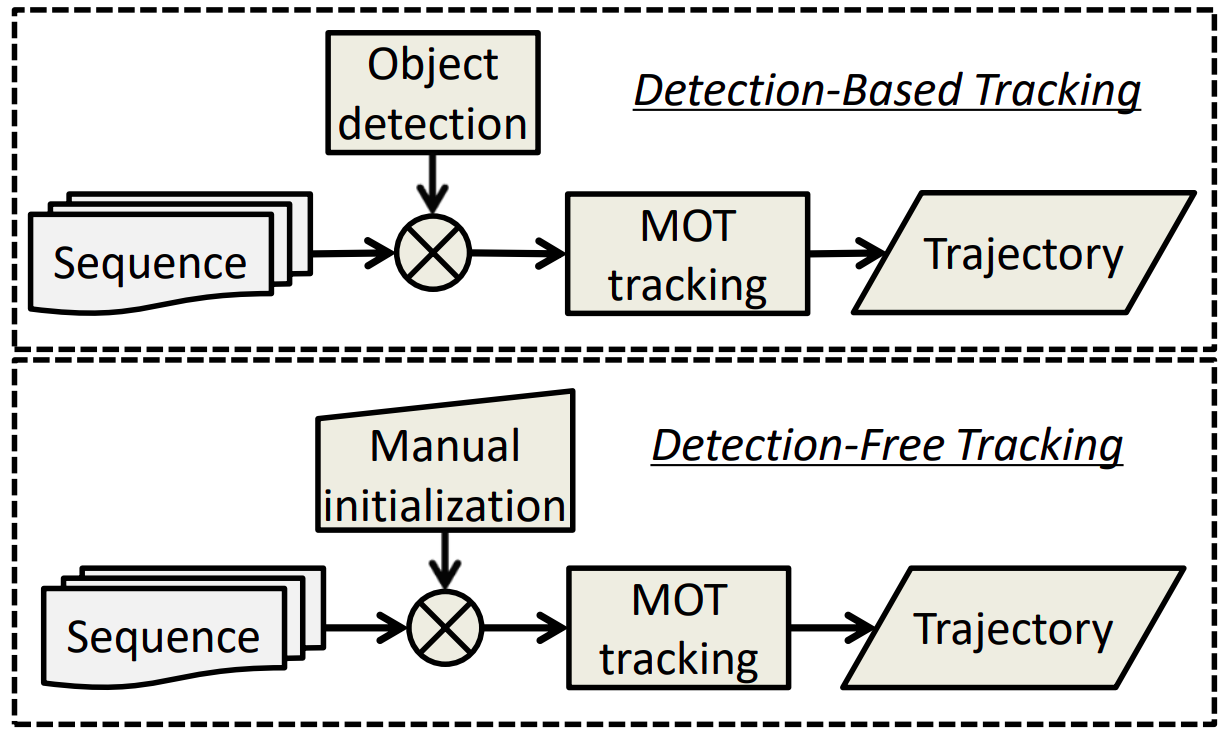
\includegraphics[width=0.6\linewidth]{img/MOT.png}
                        \caption{Pipeline of detection based tracking and detection free tracking}
                    \end{figure}
            \end{itemize}
        \item Processing mode: based on processing mode, MOT can be divided into online tracking and offline tracking problem. 
            \begin{itemize}
                \item An online model receives video input on a frame-by-frame basis, and has to give an output for each frame. This means that, in addition to the current frame, 
                only information from past frames can be used. Online tracking takes up-to-time observation and updates trajectories on the fly there for it is suitable for real time application.
                \item Offline models, on the other hand, have access to the entire video, which means that information from both past and future frames can be used. The task can then be viewed as an 
                optimization problem, where the goal is to find a set of paths that minimize some global loss  function. Offline tracking takes a batch of frames to process therefore it products delay results. 
                Since offline trackers have access to more information, one can expect better performance from these models. 
            \end{itemize}
    \end{itemize}
    Detection free tracking process data sequentially while in Detection based tracking, tracklet or detection response are often associated in batch. \\ 
    \vspace{3mm}
    Recently with the rise of deep learning, MOT can also devided into non-deep learning based methods and deep learning based methods. \\ 
    \vspace{3mm}
    In deep learning based methods, first CNN-based object detectors are applied such as Faster R-CNN and YOLOv3 to localize all objects of interest in input images. Then in a separate step,they crop the images 
    according to the boxes and feed them to an identity embedding network to extract re-ID features which are used to link the boxes over time. The linking step usually follows a standard practice which first 
    computes a cost matrix according to the re-ID features and Intersection over Unions (IoU) of the bounding boxes and then uses the Kalman Filter and Hungarian algorithm to accomplish the linking task. 
    MOT methods based on deep learning can be further devided into two-stage method and one-stage method. \\ 
    \vspace{3mm}
    The main advantage of the two-step methods is that they can develop the most suitable model for each task separately without making compromise. In addition, they can crop the image patches according to the 
    detected bounding boxes and resize them to the same size before estimating re-ID features. This helps to handle the scale variations of objects.The main drawback due to the fact that they are usually very 
    slow because the two tasks need to be done separately without sharing. \\ 
    \vspace{3mm}
    For one stage method, the core idea is to simultaneously accomplish object detection and identity embedding (re-ID features) in a single network in order to reduce inference time. However, the accuracy of the 
    one-shot trackers is usually lower than that of the two-step ones.

\section{MOT Components Overview}
    \subsection{Appearance Model}
        Appearance model includes visual representation and statistical measuring. Appearance model is important cue for affinity computation in MO. Visual representation: local features, region features, 
        Probabilistic Occupancy Map (POM), depth features, Statistical measuring: single cue \& multiple cues (five kinds of fusion strategies: Boosting, Concatenating, Summation, Product, and Cascading).
    \subsection{Motion Model}
        Motion model includes linear \& non-linear model. It aims to estimates the potential position of objects in the future frames, thereby reducing the search space.
    \subsection{Interaction Model} 
        Interaction model, also known as mutual motion model, captures the influence of an object on other objects. In the crowd scenery, an object would experience some “force” from other agents and objects. 
        Interaction model includes social force model \& crowd motion pattern model.
    \subsection{Exclusion Model}
        Exclusion model includes detection-level exclusion \& trajectory-level exclusion. Exclusion is a constraint employed to avoid physical collisions when seeking a solution to the MOT problem. It arises from 
        the fact that two distinct objects cannot occupy the same physical space in the real world.
    \subsection{Occlusion Handling}
        Occlusion is perhaps the most critical challenge in MOT. It is a primary cause for ID switches or fragmentation of trajectories. In order to handle occlusion, various kinds of strategies have been proposed such as: 
        part-to-whole, hypothesize-and-test, buffer-and-recover.
    \subsection{Inference Models}
        \begin{itemize}
            \item \textbf{Probabilistic Inference} \\ 
                Approaches based on probabilistic inference typically  represent states of objects as a distribution with uncertainty. The goal of a tracking algorithm is to estimate the probabilistic distribution of target state 
                by a variety of probability reasoning methods based on existing observations. This kind of approach typically requires only the existing, i.e. past and present observations, thus they are especially appropriate for 
                the task of online tracking. \\
                \vspace{3mm}
                Although the probabilistic approaches provide a more intuitive and complete solution to the problem, they are usually difficult to infer.
                \subsection{Bayesian Estimation}
                    Bayesian estimation refers to the task of recursively estimating the state \textbf{$x_t$} at time k, from observations \emph{$z_k$}, where \emph{$z_k$} are the measurements obtained up to and including time k 
                    The algorithm of estimating the state is divided into two steps, the time update step (also called prediction) and the measurement update step. Commonly used algorithms/filters to perform the Bayesian estimation 
                    are different variations of the Kalman Filter (KF), such as Extended KF and Unscented KF. One can also use Monte Carlo samples, so called Particle filters. The choice of filter is dependent on the type of distributions 
                    and the nonlinearities and uncertainties of the motion and measurement models.
                    \begin{figure}[H]
                        \centering
                        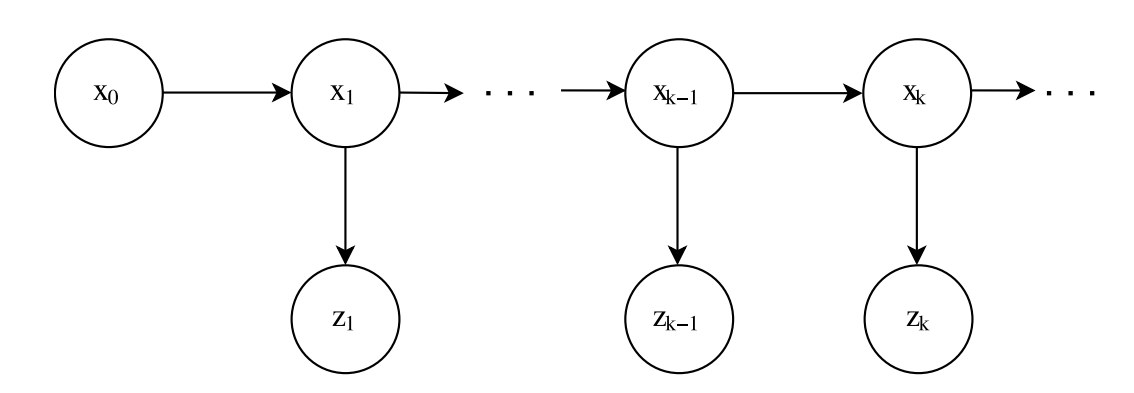
\includegraphics[width=0.6\linewidth]{img/Bayesian.png}
                        \caption{Illustration of Bayesian filtering and dependencies on time and measurement updates}
                    \end{figure}
                    \subsubsection{Time Update}
                        In the time update step, the idea is to predict the state \textbf{$x_k$} given measurements up to time k - 1, and \emph{$z^{k-1}$} this is commonly done using the Chapman–Kolmogorov equation
                        \begin{align}
                            p(x_k | z^{k-1}) = \int p(x_k | x_{k-1}) p(x_{k-1} | z^{k-1}) d x_{k-1}
                        \end{align} 
                        The transition density \emph{$p(x_k | x_{k-1})$} is defined from the choice of the motion models \textbf{$x_k = f(x_{k-1}, v_{k-1})$} where \emph{$v_k$} is a random noise process included in order to handle 
                        uncertainties and model errors. Namely the time update predicts the motion of the object.
                    \subsubsection{Measurement Update}
                        The predicted state is updated with the information from the measurement at time k. The connection between the state and the measurement is given by a measurement model \emph{$z_k = h(x_k,w_k)$}, where \emph{$w_k$} is noise. 
                        The measurement model gives rise to the likelihood of the measurement \emph{$p(z_k | x_k)$}. Since the state is estimated, it is common that the state is described by its distribution. Thus, it also includes information about 
                        the uncertainty of the estimation. We denote the prediction distribution \emph{$p_{k | k-1}(x_k | z^{k-1})$} and the posterior distribution \emph{$p_{k | k}(x_k | z^{k})$}. Subscript k | k - 1 means that the variable was 
                        computed for time \emph{k} given measurement up to time \emph{k - 1}. Similarity \emph{k | k} where measurements up to time k was used. From Bayes' theorem it follows that:
                        \begin{align}
                            p_{k|k} (x_k|z^k) \propto p(z^k|x_k) p(x_k) \propto p(z_k|x_k) p_{k|k-1} (x_k|z^{k-1})
                        \end{align}
                    \subsubsection{Kalman Filter}
                        Kalman filters have a wide variety of applications. Some of the most common applications are navigation and control for vehicles, radar tracking for anti-ballistic missiles, process control, etc. \\
                        \vspace{3mm}
                        Kalman Filter is a way of recursively finding the Bayesian estimate $\hat{x_k}$ of the true state \emph{x}. Thus it is usually more accurate than filters that compute their estimates using only the current measurement. 
                        First, at time k, a prediction is made according to the Chapman–Kolmogorov equation. When a new measurement is received, an update of said prediction is calculated based on Bayes’ theorem. How much the update relies on 
                        the prediction and the new measurement is determined by the Kalman gain, which is a way to weight the two update steps against each other, depending on their respective uncertainty. It can be shown that the (linear) 
                        Kalman filter is optimal (in the sense of minimizing the mean square error) in the cases where the noise is Gaussian.
                        \begin{figure}[H]
                            \centering
                            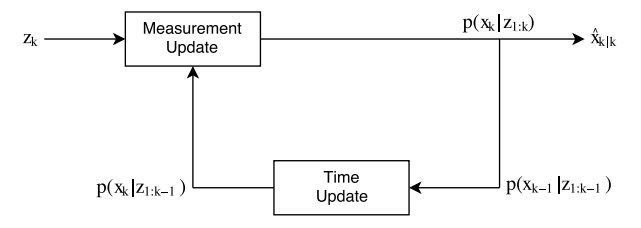
\includegraphics[width=0.6\linewidth]{img/time-measurement.png}
                            \caption{Time and measurement update}
                        \end{figure}
                            \begin{enumerate}
                                \item \textbf{Time Update} \\ 
                                    \vspace{3mm}
                                    As mentioned, during the time update step a prediction of the state is performed using a motion model \emph{$f(\hat{x_{k-1}}, v_{k-1})$}. In the case of linear motion 
                                    \begin{align}
                                        x_k = F_{k-1} X_{k-1 | k-1} + q_{k-1}
                                    \end{align}
                                    The time update of the mean and covariance can be computed as 
                                    \begin{align}
                                        \hat{x}_{k|k-1} = F_{k-1} \hat{x}_{k-1|k-1} \\ 
                                        P_{k|k-1} = F_{k-1} P_{k-1|k-1} F_{k-1}^T + Q_{k-1}
                                    \end{align}
                                    where \emph{$Q_{k-1}$} is the process noise covariance at time k-1
                                \item \textbf{Measurement Update} \\ 
                                    \vspace{3mm}
                                    Given a new measurement \emph{$z_k$} at time \emph{k} with measurement covariance \emph{$R_k$} we can update the predicted state. In the case of linear measurement models and independent Gaussian noise, 
                                    we can describe the measurement model \emph{$z_k = h(\hat{x_k}, w_k)$} as
                                    \begin{align}
                                        z_k = H_k x_k + w_k
                                    \end{align}  
                                    The update equations of Kalman Filter are 
                                    \begin{align}
                                        \hat{x}_k|k = \hat{x}_{k|k-1} + K_k v_k
                                        P_{k|k} = P_{k|k-1} - K_k S_k K_k^T
                                    \end{align}
                                    where the Kalman gain \emph{$K_k$} innovation \emph{$v_k$}, the innovation covariance, \emph{$S_k$} at time \emph{k} are
                                    \begin{align}
                                        K_k = P_{k|k-1} H_k^T S_k^{-1}
                                        v_k = z_k - H_k \hat{x}_{k|k-1}
                                        S_k = H_k P_{k|k-1} H_k^T + R_k
                                    \end{align}
                                    The innovation captures the new information that the new measurement brings and the Kalman gain determines how much we should rely on this information.
                            \end{enumerate}
                    \subsubsection{Unscented Kalman Filter}
                        The Kalman filter is derived from linear models, thus is only optimal for this case and not for nonlinear models. If the models are nonlinear, linearization can be used, known as the Extended Kalman Filter (EKF). 
                        The EKF works well in many cases, although it may perform poorly if the model is significantly nonlinear within the uncertainties of the models. However, there are other methods of solving the estimation task that 
                        are more robust to nonlinearities. The derivation of the Kalman filter contains multiple integrals of the type
                        \begin{align}
                            \int g(x) \mathcal{N} (x;\hat{x};P) dx = E [g(x)]
                        \end{align}
                        where E denotes the expected value. Furthermore \emph{g(x)} is either a motion or measurement model, which can be non linear. Integrals for example in the Chapman-Kolmogorov equation may look like 
                        \begin{align}
                            \int g(x_{k-1}) \mathcal{N} (x_{k-1}; \hat{x}_{k-1|k-1}; P_{k-1|k-1}) dx_{k-1}
                        \end{align}
                        These integrals can be solved for linear models, however with nonlinear models this is not the case. Thus, these integrals needs to be approximated, one way of doing so is to use the Monte Carlo method. 
                        The idea is to generate independent and identicallyy distributed samples $x^{(1)},x^{(2)},...,x^{(N)}$ from its distribution \emph{p(x)}, that we can approximate
                        \begin{align}
                            \int g(x) p(x) dx \approx \frac{1}{N} \displaystyle\sum_{i=1}^N g(x_{(i)})
                        \end{align}
                        However as the Monte Carlo method relies on picking random samples, it might require a lot of samples in order to represent the true distribution. As an alternative, there are so called $\sigma$ -point methods which use 
                        deterministic samples chosen in clever ways to cover a large area of the space even though the number of samples is small. We will focus on one of these, the so called Unscented Kalman Filter (UKF). Two advantages of this 
                        filter are that it is efficient since it uses quite few samples, and it also only has one tuning parameter.
                            \begin{enumerate}
                                \item \textbf{Time Update} \\ 
                                    \vspace{3mm}
                                    With a state vector \emph{$x_k$} of dimension \emph{n}, the idea is to generate \emph{2n + 1} $\sigma$-point $\mathcal{X}$
                                    \begin{align}
                                        \mathcal{X}_{k-1}^{(0)} = \hat{x}_{k-1|k-1} \\
                                        \mathcal{X}_{k-1}^{(i)} = \hat{x}_{k-1|k-1} + \sqrt{\frac{n}{1-W_0}} P_{i,k-1|k-1}^{1/2} & with i = 1,2,...,n \\
                                        \mathcal{X}_{k-1}^{(i+n)} = \hat{x}_{k-1|k-1} - \sqrt{\frac{n}{1-W_0}} P_{i,k-1|k-1}^{1/2} & with i = 1,2,...,n 
                                    \end{align}
                                    where \emph{$W_0$} is the tuning parameter (namely the weight of $\mathcal{X}$). \textbf{$P^{(1/2)}$} is the matrix such that
                                    \begin{align}
                                        P = P^{(1/2)} (P^{(1/2)})^T
                                    \end{align}
                                    and \emph{$P_i^(1/2)$} is its \emph{ith} column. The UKF prediction equations are then given by
                                    \begin{align}
                                        \hat{x}_{k|k-1} = \displaystyle\sum_{i=0}^{2n} f(\mathcal{X}_{k-1}^{(i)}) W_i \\
                                        P_{k|k-1} = Q_{k-1} + \displaystyle\sum_{i=0}^{2n} (f(\mathcal{X}_{k-1}^{(1)}) - \hat{x}_{k|k-1}) (.)^T W_i
                                    \end{align} 
                                    where $W_i = \frac{1-W_0}{2n}$ for i = 1,2,...,n.
                                \item \textbf{Measurement Update} \\ 
                                    Similarly, in the measurement update step, the $\sigma$-points are chosen to 
                                    \begin{align}
                                        \mathcal{X}_k^{(0)} = \hat{x}_{k|k-1}
                                    \end{align}
                            \end{enumerate}
        \end{itemize}


\section{Detection Based Tracking Pipeline}

\section{SORT}

\section{Deep SORT}

\section{Evaluations Metrics}

    \subsection{Conventional Metrics}

    \subsection{Update Metrics}